\documentclass[tikz,border=10pt]{standalone}

\usepackage{tikz}
\usepackage{amssymb,amsmath,amsthm,amsfonts}

\newcommand{\ket}[1]{\left| #1 \right \rangle}

\begin{document}


%%%FIGURA SFERA DI BLOCH PER H %%%
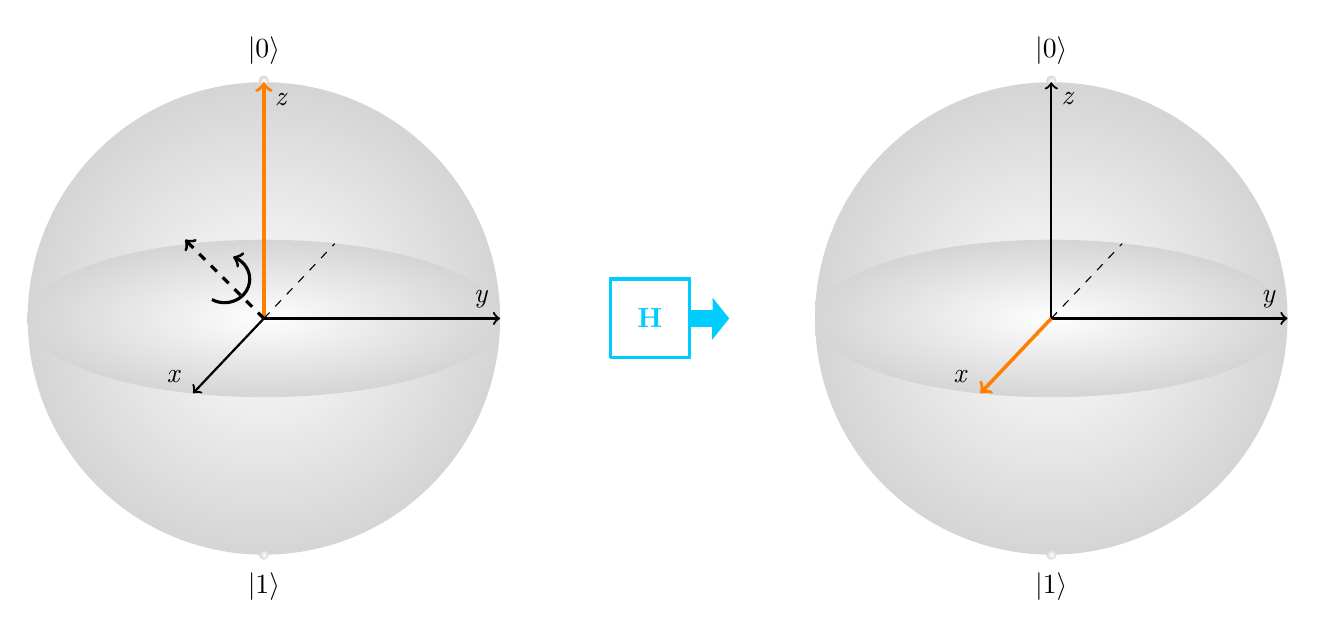
\begin{tikzpicture}

\draw[dashed] (3,3) -- (3,0);

\shade[inner color={rgb:black,1;white,200} ,outer color={rgb:black,1;white,5}  ] (3,3) circle (3cm);
\shade[inner color={rgb:black,1;white,200} ,outer color={rgb:black,1;white,5}  ]  (3,3) ellipse (3cm and 1cm);
%\draw (3,3) circle (3cm);
%\draw[dashed, color={rgb:black,1;white,2}] (3,3) ellipse (3cm and 1cm);

\shade[inner color={rgb:black,1;white,200} ,outer color={rgb:black,1;white,5}  ] (3,6.02) circle (0.065cm);

\draw (3,6.1) node[anchor=south] {\textit{$ \ket{0}$}} ;
\draw (3,-0.1) node[anchor=north] {\textit{$ \ket{1}$}} ;

\draw[color=orange,line width=0.45mm,->] (3,3) -- (3,6)  node[text=black,anchor=north west] {\textit{z}} ;
\draw[thick,->] (3,3) -- (6,3) node[anchor= south east] {\textit{y}} ;
\draw[color=black,thick,->] (3,3) -- (2.1,2.05) node[text=black,anchor= south east] {\textit{x}} ;

\draw[dashed] (3,3) -- (3.9,3.95)  ;

\shade[inner color={rgb:black,1;white,200} ,outer color={rgb:black,1;white,5}  ] (3,0) circle (0.065cm);

%%%%

\definecolor{yucky}{HTML}{00CCFF}

\coordinate (birds) at (8-0.1,3);
\node[text=yucky] at (birds) {\textbf{H}};

\draw[line width=0.40mm, color=yucky] (7.5-0.1,2.5) -- (8.5-0.1,2.5) -- (8.5-0.1,3.5) -- (7.5-0.1,3.5) -- (7.5-0.1,2.5) ;

%freccia
\filldraw[ color=yucky] (8.5-0.1,2.9) -- (8.8-0.1,2.9) -- (8.8-0.1,3.1) -- (8.5-0.1,3.1) -- (8.5-0.1,2.9) ;

\filldraw[ color=yucky] (8.8-0.1,2.9) -- (8.8-0.1,2.75) --  (9-0.1,3) -- (8.8-0.1,3.25);

%%%SFERA TRASLATA%%
\draw[dashed] (3+10,3) -- (3+10,0);

\shade[inner color={rgb:black,1;white,200} ,outer color={rgb:black,1;white,5}  ] (3+10,3) circle (3cm);
\shade[inner color={rgb:black,1;white,200} ,outer color={rgb:black,1;white,5}  ]  (3+10,3) ellipse (3cm and 1cm);
%\draw (3,3) circle (3cm);
%\draw[dashed, color={rgb:black,1;white,2}] (3,3) ellipse (3cm and 1cm);

\shade[inner color={rgb:black,1;white,200} ,outer color={rgb:black,1;white,5}  ] (3+10,6.02) circle (0.065cm);

\draw (3+10,6.1) node[anchor=south] {\textit{$ \ket{0}$}} ;
\draw (3+10,-0.1) node[anchor=north] {\textit{$ \ket{1}$}} ;

\draw[color=black,thick,->] (3+10,3) -- (3+10,6)  node[text=black,anchor=north west] {\textit{z}} ;

\draw[thick,->] (3+10,3) -- (6+10,3) node[anchor= south east] {\textit{y}} ;
\draw[color=orange,line width=0.45mm,->] (3+10,3) -- (2.1+10,2.05) node[text=black,anchor= south east] {\textit{x}} ; 

\draw[dashed] (3+10,3) -- (3.9+10,3.95)  ;

\shade[inner color={rgb:black,1;white,200} ,outer color={rgb:black,1;white,5}  ] (3+10,0) circle (0.065cm);



%%rotazione
\draw [line width=0.40mm,domain=-120:70,->] plot ({2.5 + 0.32*cos(\x)}, {3.5 + 0.3*sin(\x)});
\draw [dashed,line width=0.40mm,->] (3,3) -- (2,4);

\end{tikzpicture}




\end{document}